\documentclass[10pt]{article}
\usepackage[left=0.9in,top=0.9in,bottom=0.9in,right=0.9in]{geometry}
\usepackage[english]{babel}
\usepackage{fancyhdr}
\usepackage{lastpage}
\usepackage{caption}
\usepackage{amsmath}
\usepackage{hyperref}
\usepackage{xcolor}
\usepackage{graphicx}
\usepackage{float}
\usepackage{textcomp}
\usepackage{amssymb}
\usepackage{mathrsfs}
\usepackage{soul}
\usepackage{enumerate}
\usepackage{wrapfig}
\usepackage{listings}
\usepackage{diagbox}
\usepackage{multirow}

% Listings settings
\lstset{frame=tb,
  language=Python,
  aboveskip=3mm,
  belowskip=3mm,
  showstringspaces=false,
  columns=flexible,
  basicstyle={\scriptsize\ttfamily},
  breaklines=true,
  breakatwhitespace=true,
  tabsize=3,
  numbers=left,
  xleftmargin=4em,
  framexleftmargin=3.5em
}

% Remove bibliography title
\usepackage{etoolbox}
\patchcmd{\thebibliography}{\section*{\refname}}{}{}{}

% Set up header/footers
\pagestyle{fancy}
\fancyhead[LE,RO]{\today}
\fancyhead[C]{NE 255 - HW 6}
\fancyhead[LO,RE]{D. Hellfeld}
\fancyfoot[C]{\thepage\ of \pageref{LastPage}}
\renewcommand{\headrulewidth}{0.4pt}
\renewcommand{\footrulewidth}{0.4pt}

% Set up figure/table captions \textbf{}
\addto\captionsenglish{\renewcommand{\figurename}{Fig.}}
\addto\captionsenglish{\renewcommand{\tablename}{\small Table}}
%\renewcommand{\thetable}{\Roman{table}}
\captionsetup[table]{labelfont = normal, labelsep=period, singlelinecheck=true}
\captionsetup[figure]{labelfont=normal, labelsep=period, singlelinecheck=true}

% Remove paragraph indent
\setlength\parindent{0pt}


\begin{document}


% - - - - - - - - - - - - - - - - - - - - - - - - - - - - - - - - - - - - - - - - - -
\begin{centering}
\textbf{\large NE 255 - Homework 6}\\
\vspace{10pt}
University of California, Berkeley\\
Department of Nuclear Engineering\\
\vspace{10pt}
Daniel Hellfeld\\
\href{mailto:dhellfeld@berkeley.edu}{dhellfeld@berkeley.edu}\\
\end{centering}






% - - - - - - - - - - - - - - - - - - - - - - - - - - - - - - - - - - - - - - - - - -
\vspace{20pt}
\noindent \textbf{Problem 1}\\
Using the direct inversion of CDF sampling method, derive sampling algorithms for

\begin{enumerate}[(a)]
	\item The neutron direction in 3D if the neutron source is isotropic.
\end{enumerate}

...

%
%
%

\begin{enumerate}[(b)]
	\item The distance to the next collision in the direction of neutron motion if the neutron is in the center of the spherical volume that consists of three concentric layers with radii $R_1$, $R_2$, and $R_3$, each made of different materials with total cross sections $\Sigma_{t1}$, $\Sigma_{t2}$, and $\Sigma_{t3}$, respectively.
\end{enumerate}

...

%
%
%

\begin{enumerate}[(c)]
	\item The type of collision if it is assumed that the neutron can have both elastic and in-elastic scattering, and can be absorbed in fission or ($n$,$\gamma$) capture interactions. Assume monoenergetic neutron transport.
\end{enumerate}

...

%
%
%

% - - - - - - - - - - - - - - - - - - - - - - - - - - - - - - - - - - - - - - - - - -
\newpage
\noindent \textbf{Problem 2}\\
Use a rejection Monte Carlo method to evaluate $\pi = 3.14159$:

\begin{itemize}
	\item From $\pi = 4 \int_0^1 \sqrt{1-x^2} dx$
	\item From $\pi = 4 \int_0^1 \frac{1}{1+x^2} dx$
	\item Assuming the $\pi = 3.14159$ is exact, calculate the relative error for 10, 100, 1,000, and 10,000 samples.
	\item What do you notice about the behavior of error as a function of the number of trials?
\end{itemize}

$\Rightarrow$ A code was written in Python to perform the rejection sampling and calculate $\pi$ using the two functions above. The relative error is also calculated for the different number of samples for each function. The results were then also fit to a function of the form

\begin{equation*}
	f(x) = \frac{a}{\sqrt{N}}
\end{equation*}

and plotted together. This is because we expect the relative error to decrease with the number of samples as $1/\sqrt{N}$. The code is shown below and the relative error results (for both functions) are tabulated in Table 1 and plotted in Fig.~1 with the fitted function.\\

\lstinputlisting[language=Python]{../p2/p2.py}

\begin{table}[htb!]
\centering
\begin{tabular}{|c|c|c|c|c|}
\hline
\multirow{2}{*}{Number of Samples (N)} & \multicolumn{2}{c|}{Function 1: $4\sqrt{1-x^2}$} & \multicolumn{2}{c|}{Function 2: $4/(1+x^2)$} \\ \cline{2-5}
& Estimated value & Relative Error (\%) & Estimated value & Relative Error (\%) \\ \hline
10         & 2.9400 & 6.4168 & 2.9400 & 6.4168 \\ \hline
50         & 2.8560 & 9.0906 & 2.9400 & 6.4168 \\ \hline
100       & 3.2760 & 4.2784 & 3.3600 & 6.9522 \\ \hline
500       & 3.0912 & 1.6039 & 3.1584 & 0.5350 \\ \hline
1000     & 3.0576 & 2.6734 & 3.0828 & 1.8713 \\ \hline
5000     & 3.1609 & 0.6152 & 3.1668 & 0.8024 \\ \hline
10000   & 3.1214 & 0.6413 & 3.1227 & 0.6012 \\ \hline
50000   & 3.1399 & 0.0531 & 3.1427 & 0.0377 \\ \hline
100000 & 3.1433 & 0.0551 & 3.1458 & 0.1353 \\ \hline
\end{tabular}
\caption{Rejection sampling estimate and relative errors for $\pi = 3.14159$ using two different functions.}
\end{table}

\begin{figure}[H]
\centering
\begin{tabular}{cc}
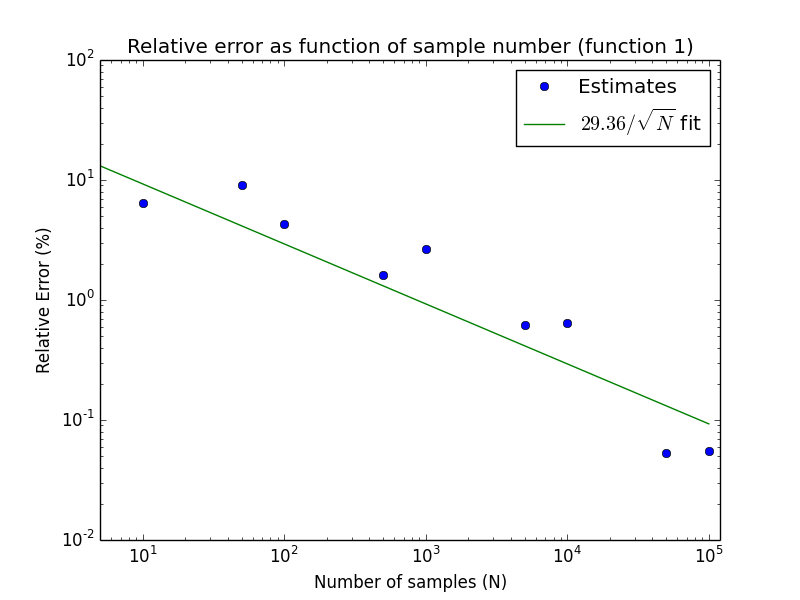
\includegraphics[height=170pt]{Figures/function1.png} & 
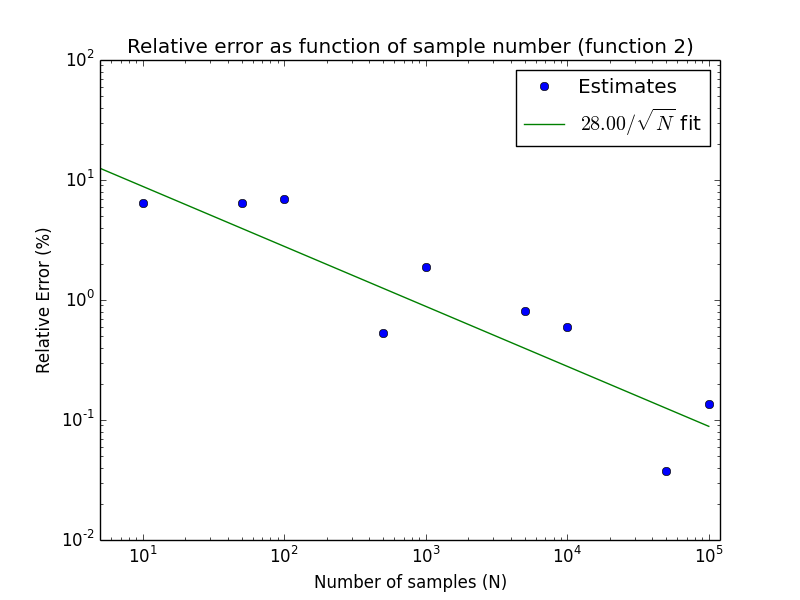
\includegraphics[height=170pt]{Figures/function2.png} \\
\footnotesize{(a)} & \footnotesize{(b)}
\end{tabular}
\caption{(a) Relative errors as function of sample number for function 1, plotted with fit line. (b) Relative errors as function of sample number for function 2, plotted with fit line.}
\end{figure}              

We see that the relative errors generally decrease as the sample number is increased. Of course there is some variation because we are using random numbers. However, in both cases, we observe that the general trend of the relative errors seems to follow the expected $\propto N^{-1/2}$ behavior.
           
    
% - - - - - - - - - - - - - - - - - - - - - - - - - - - - - - - - - - - - - - - - - -

\end{document}
